% Options for packages loaded elsewhere
\PassOptionsToPackage{unicode}{hyperref}
\PassOptionsToPackage{hyphens}{url}
%
\documentclass[
]{article}
\usepackage{amsmath,amssymb}
\usepackage{lmodern}
\usepackage{iftex}
\ifPDFTeX
  \usepackage[T1]{fontenc}
  \usepackage[utf8]{inputenc}
  \usepackage{textcomp} % provide euro and other symbols
\else % if luatex or xetex
  \usepackage{unicode-math}
  \defaultfontfeatures{Scale=MatchLowercase}
  \defaultfontfeatures[\rmfamily]{Ligatures=TeX,Scale=1}
\fi
% Use upquote if available, for straight quotes in verbatim environments
\IfFileExists{upquote.sty}{\usepackage{upquote}}{}
\IfFileExists{microtype.sty}{% use microtype if available
  \usepackage[]{microtype}
  \UseMicrotypeSet[protrusion]{basicmath} % disable protrusion for tt fonts
}{}
\makeatletter
\@ifundefined{KOMAClassName}{% if non-KOMA class
  \IfFileExists{parskip.sty}{%
    \usepackage{parskip}
  }{% else
    \setlength{\parindent}{0pt}
    \setlength{\parskip}{6pt plus 2pt minus 1pt}}
}{% if KOMA class
  \KOMAoptions{parskip=half}}
\makeatother
\usepackage{xcolor}
\usepackage[margin=1in]{geometry}
\usepackage{color}
\usepackage{fancyvrb}
\newcommand{\VerbBar}{|}
\newcommand{\VERB}{\Verb[commandchars=\\\{\}]}
\DefineVerbatimEnvironment{Highlighting}{Verbatim}{commandchars=\\\{\}}
% Add ',fontsize=\small' for more characters per line
\usepackage{framed}
\definecolor{shadecolor}{RGB}{248,248,248}
\newenvironment{Shaded}{\begin{snugshade}}{\end{snugshade}}
\newcommand{\AlertTok}[1]{\textcolor[rgb]{0.94,0.16,0.16}{#1}}
\newcommand{\AnnotationTok}[1]{\textcolor[rgb]{0.56,0.35,0.01}{\textbf{\textit{#1}}}}
\newcommand{\AttributeTok}[1]{\textcolor[rgb]{0.77,0.63,0.00}{#1}}
\newcommand{\BaseNTok}[1]{\textcolor[rgb]{0.00,0.00,0.81}{#1}}
\newcommand{\BuiltInTok}[1]{#1}
\newcommand{\CharTok}[1]{\textcolor[rgb]{0.31,0.60,0.02}{#1}}
\newcommand{\CommentTok}[1]{\textcolor[rgb]{0.56,0.35,0.01}{\textit{#1}}}
\newcommand{\CommentVarTok}[1]{\textcolor[rgb]{0.56,0.35,0.01}{\textbf{\textit{#1}}}}
\newcommand{\ConstantTok}[1]{\textcolor[rgb]{0.00,0.00,0.00}{#1}}
\newcommand{\ControlFlowTok}[1]{\textcolor[rgb]{0.13,0.29,0.53}{\textbf{#1}}}
\newcommand{\DataTypeTok}[1]{\textcolor[rgb]{0.13,0.29,0.53}{#1}}
\newcommand{\DecValTok}[1]{\textcolor[rgb]{0.00,0.00,0.81}{#1}}
\newcommand{\DocumentationTok}[1]{\textcolor[rgb]{0.56,0.35,0.01}{\textbf{\textit{#1}}}}
\newcommand{\ErrorTok}[1]{\textcolor[rgb]{0.64,0.00,0.00}{\textbf{#1}}}
\newcommand{\ExtensionTok}[1]{#1}
\newcommand{\FloatTok}[1]{\textcolor[rgb]{0.00,0.00,0.81}{#1}}
\newcommand{\FunctionTok}[1]{\textcolor[rgb]{0.00,0.00,0.00}{#1}}
\newcommand{\ImportTok}[1]{#1}
\newcommand{\InformationTok}[1]{\textcolor[rgb]{0.56,0.35,0.01}{\textbf{\textit{#1}}}}
\newcommand{\KeywordTok}[1]{\textcolor[rgb]{0.13,0.29,0.53}{\textbf{#1}}}
\newcommand{\NormalTok}[1]{#1}
\newcommand{\OperatorTok}[1]{\textcolor[rgb]{0.81,0.36,0.00}{\textbf{#1}}}
\newcommand{\OtherTok}[1]{\textcolor[rgb]{0.56,0.35,0.01}{#1}}
\newcommand{\PreprocessorTok}[1]{\textcolor[rgb]{0.56,0.35,0.01}{\textit{#1}}}
\newcommand{\RegionMarkerTok}[1]{#1}
\newcommand{\SpecialCharTok}[1]{\textcolor[rgb]{0.00,0.00,0.00}{#1}}
\newcommand{\SpecialStringTok}[1]{\textcolor[rgb]{0.31,0.60,0.02}{#1}}
\newcommand{\StringTok}[1]{\textcolor[rgb]{0.31,0.60,0.02}{#1}}
\newcommand{\VariableTok}[1]{\textcolor[rgb]{0.00,0.00,0.00}{#1}}
\newcommand{\VerbatimStringTok}[1]{\textcolor[rgb]{0.31,0.60,0.02}{#1}}
\newcommand{\WarningTok}[1]{\textcolor[rgb]{0.56,0.35,0.01}{\textbf{\textit{#1}}}}
\usepackage{graphicx}
\makeatletter
\def\maxwidth{\ifdim\Gin@nat@width>\linewidth\linewidth\else\Gin@nat@width\fi}
\def\maxheight{\ifdim\Gin@nat@height>\textheight\textheight\else\Gin@nat@height\fi}
\makeatother
% Scale images if necessary, so that they will not overflow the page
% margins by default, and it is still possible to overwrite the defaults
% using explicit options in \includegraphics[width, height, ...]{}
\setkeys{Gin}{width=\maxwidth,height=\maxheight,keepaspectratio}
% Set default figure placement to htbp
\makeatletter
\def\fps@figure{htbp}
\makeatother
\setlength{\emergencystretch}{3em} % prevent overfull lines
\providecommand{\tightlist}{%
  \setlength{\itemsep}{0pt}\setlength{\parskip}{0pt}}
\setcounter{secnumdepth}{-\maxdimen} % remove section numbering
\ifLuaTeX
  \usepackage{selnolig}  % disable illegal ligatures
\fi
\IfFileExists{bookmark.sty}{\usepackage{bookmark}}{\usepackage{hyperref}}
\IfFileExists{xurl.sty}{\usepackage{xurl}}{} % add URL line breaks if available
\urlstyle{same} % disable monospaced font for URLs
\hypersetup{
  pdftitle={Lab 2 Analyzing multivariate salmon data},
  pdfauthor={E Holmes},
  hidelinks,
  pdfcreator={LaTeX via pandoc}}

\title{Lab 2 Analyzing multivariate salmon data}
\author{E Holmes}
\date{April 13, 2023}

\begin{document}
\maketitle

{
\setcounter{tocdepth}{2}
\tableofcontents
}
\begin{Shaded}
\begin{Highlighting}[]
\FunctionTok{library}\NormalTok{(tidyverse)}
\FunctionTok{options}\NormalTok{(}\AttributeTok{dplyr.summarise.inform =} \ConstantTok{FALSE}\NormalTok{)}
\end{Highlighting}
\end{Shaded}

For this lab you will use multivariate auto-regressive state-space
(MARSS) to analyze multivariate salmon data from the Columbia River.
These data are noisy and gappy. They are estimates of total spawner
abundance and might include hatchery spawners.

\hypertarget{teams}{%
\subsection{Teams}\label{teams}}

\begin{enumerate}
\def\labelenumi{\arabic{enumi}.}
\tightlist
\item
  Lower Columbia River Chinook: Zoe Rand (QERM), Emma Timmins-Schiffman
  (Genome Sci), Maria Kuruvilla (QERM)
\item
  Lower Columbia River Steelhead: Eric French (Civil), Liz Elmstrom
  (SAFS), Terrance Wang (SAFS)
\item
  Lower Columbia River Coho: Nick Chambers (SAFS), Karl Veggerby (SAFS),
  Miranda Mudge (Molecular \& Cellular)
\item
  Middle Columbia River Steelhead: Madison Shipley (SAFS), Dylan Hubl
  (Env \& Forest Sci)
\end{enumerate}

\hypertarget{lower-columbia-river-salmon-spawner-data}{%
\subsection{Lower Columbia River salmon spawner
data}\label{lower-columbia-river-salmon-spawner-data}}

These data are from the
\href{https://www.streamnet.org/cap/about-cap/}{Coordinated Assessments
Partnership (CAP)} and downloaded using the
\href{https://nwfsc-math-bio.github.io/rCAX/}{rCAX R client} for the CAX
(the CAP database) API. The data are saved in
\texttt{Lab-2/Data\_Images/columbia-river.rda}.

\begin{Shaded}
\begin{Highlighting}[]
\FunctionTok{load}\NormalTok{(here}\SpecialCharTok{::}\FunctionTok{here}\NormalTok{(}\StringTok{"Lab{-}2"}\NormalTok{, }\StringTok{"Data\_Images"}\NormalTok{, }\StringTok{"columbia{-}river.rda"}\NormalTok{))}
\end{Highlighting}
\end{Shaded}

The data set has data for fi endangered and threatened ESU (Evolutionary
Significant Units) in the Lower Columbia River.

\begin{Shaded}
\begin{Highlighting}[]
\NormalTok{esu }\OtherTok{\textless{}{-}} \FunctionTok{unique}\NormalTok{(columbia.river}\SpecialCharTok{$}\NormalTok{esu\_dps)}
\NormalTok{esu}
\end{Highlighting}
\end{Shaded}

\begin{verbatim}
## [1] "Steelhead (Middle Columbia River DPS)"     
## [2] "Steelhead (Upper Columbia River DPS)"      
## [3] "Steelhead (Lower Columbia River DPS)"      
## [4] "Salmon, coho (Lower Columbia River ESU)"   
## [5] "Salmon, Chinook (Lower Columbia River ESU)"
\end{verbatim}

\begin{figure}
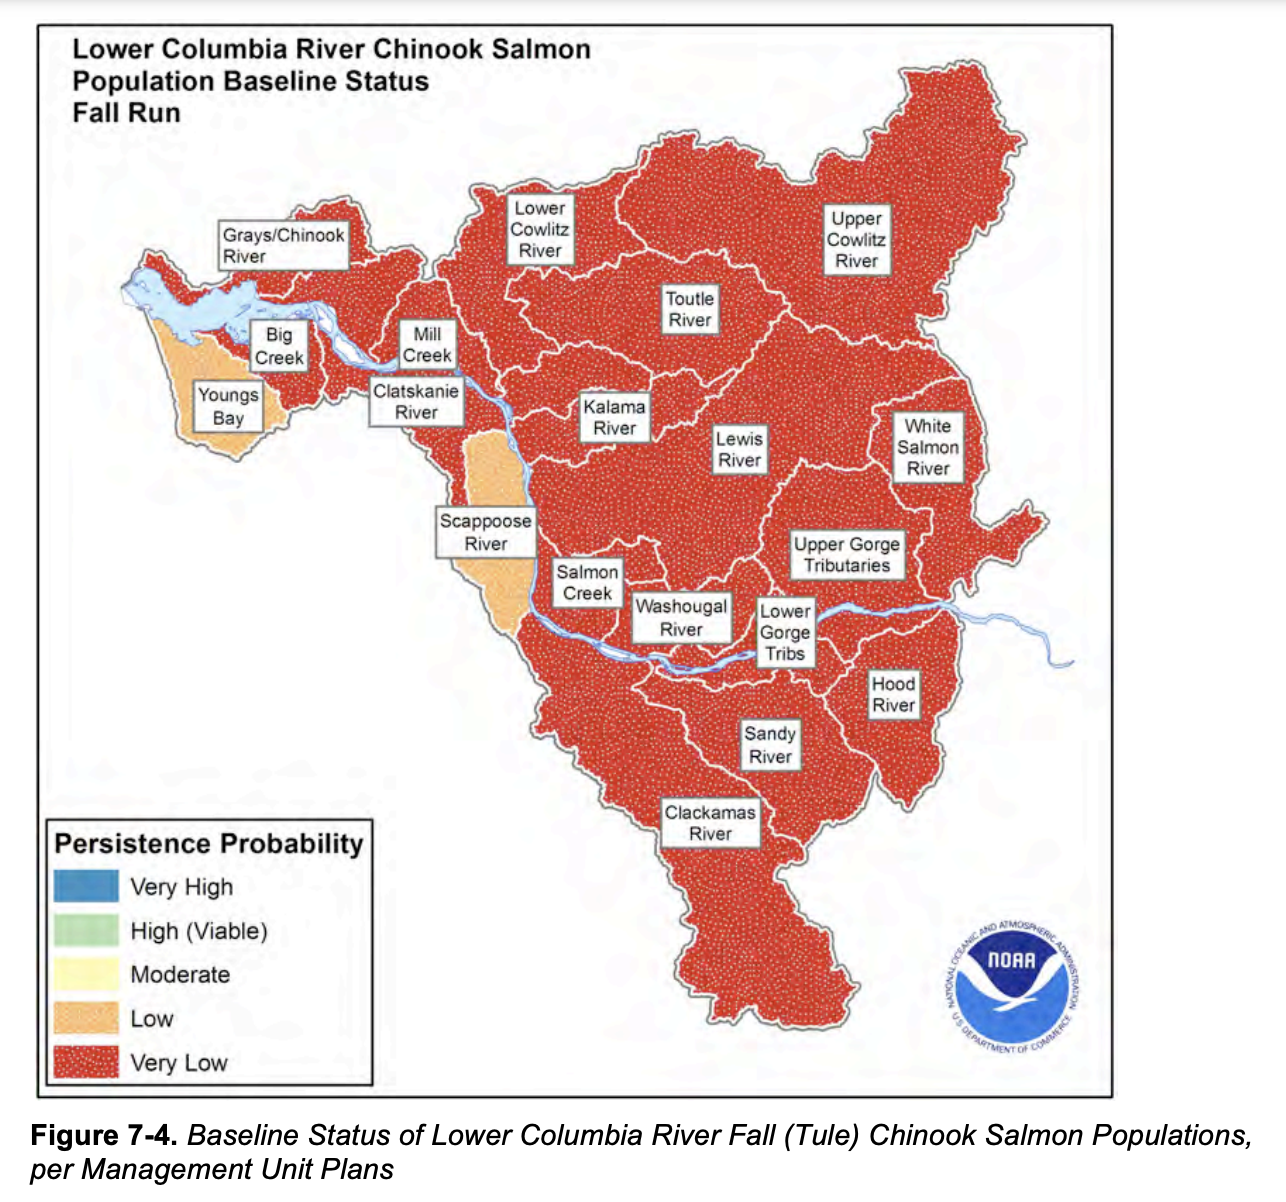
\includegraphics[width=0.5\linewidth]{Data_Images/LCR-chinook-regions} \caption{Figure from ESA recovery plan for Lower Columbia River Coho salmon, Lower Columbia River Chinook salmon, Columbia River Chum salmon, and Lower Columbia River steelhead. 2013. NMFS NW Region.  https://repository.library.noaa.gov/view/noaa/16002}\label{fig:unnamed-chunk-4}
\end{figure}

\hypertarget{data-structure}{%
\subsubsection{Data structure}\label{data-structure}}

The dataset has the following columns

\begin{Shaded}
\begin{Highlighting}[]
\FunctionTok{colnames}\NormalTok{(columbia.river)}
\end{Highlighting}
\end{Shaded}

\begin{verbatim}
## [1] "species"       "esu_dps"       "majorpopgroup" "esapopname"   
## [5] "commonpopname" "run"           "spawningyear"  "value"        
## [9] "value_type"
\end{verbatim}

\begin{itemize}
\tightlist
\item
  species: Chinook, Coho, Steelhead
\item
  esu\_dps: name of the ESU
\item
  majorpopgroup: biological major group
\item
  commonpopname: common population name, generally a stream or river
\item
  run: run-timing
\item
  spawningyear: the year that the spawners were counted on the spawning
  grounds
\item
  value: total (natural-born and hatchery-born) spawners on the spawning
  ground. Generally some type of redd-count expansion or some other
  stream count of spawners. Redd = a gravel nest.
\end{itemize}

\hypertarget{data-plots}{%
\subsubsection{Data plots}\label{data-plots}}

Let's load one ESU and make a plot. Create a function.

\begin{Shaded}
\begin{Highlighting}[]
\NormalTok{plotesu }\OtherTok{\textless{}{-}} \ControlFlowTok{function}\NormalTok{(esuname)\{}
\NormalTok{  df }\OtherTok{\textless{}{-}}\NormalTok{ columbia.river }\SpecialCharTok{\%\textgreater{}\%} \FunctionTok{subset}\NormalTok{(esu\_dps }\SpecialCharTok{\%in\%}\NormalTok{ esuname)}
\FunctionTok{ggplot}\NormalTok{(df, }\FunctionTok{aes}\NormalTok{(}\AttributeTok{x=}\NormalTok{spawningyear, }\AttributeTok{y=}\FunctionTok{log}\NormalTok{(value), }\AttributeTok{color=}\NormalTok{majorpopgroup)) }\SpecialCharTok{+} 
  \FunctionTok{geom\_point}\NormalTok{(}\AttributeTok{size=}\FloatTok{0.2}\NormalTok{, }\AttributeTok{na.rm =} \ConstantTok{TRUE}\NormalTok{) }\SpecialCharTok{+} 
  \FunctionTok{theme}\NormalTok{(}\AttributeTok{strip.text.x =} \FunctionTok{element\_text}\NormalTok{(}\AttributeTok{size =} \DecValTok{3}\NormalTok{)) }\SpecialCharTok{+}
  \FunctionTok{theme}\NormalTok{(}\AttributeTok{axis.text.x =} \FunctionTok{element\_text}\NormalTok{(}\AttributeTok{size =} \DecValTok{5}\NormalTok{, }\AttributeTok{angle =} \DecValTok{90}\NormalTok{)) }\SpecialCharTok{+}
  \FunctionTok{facet\_wrap}\NormalTok{(}\SpecialCharTok{\textasciitilde{}}\NormalTok{esapopname) }\SpecialCharTok{+}
  \FunctionTok{ggtitle}\NormalTok{(}\FunctionTok{paste0}\NormalTok{(esuname, }\AttributeTok{collapse=}\StringTok{"}\SpecialCharTok{\textbackslash{}n}\StringTok{"}\NormalTok{))}
\NormalTok{\}}
\end{Highlighting}
\end{Shaded}

\begin{Shaded}
\begin{Highlighting}[]
\FunctionTok{plotesu}\NormalTok{(esu[}\DecValTok{3}\NormalTok{])}
\end{Highlighting}
\end{Shaded}

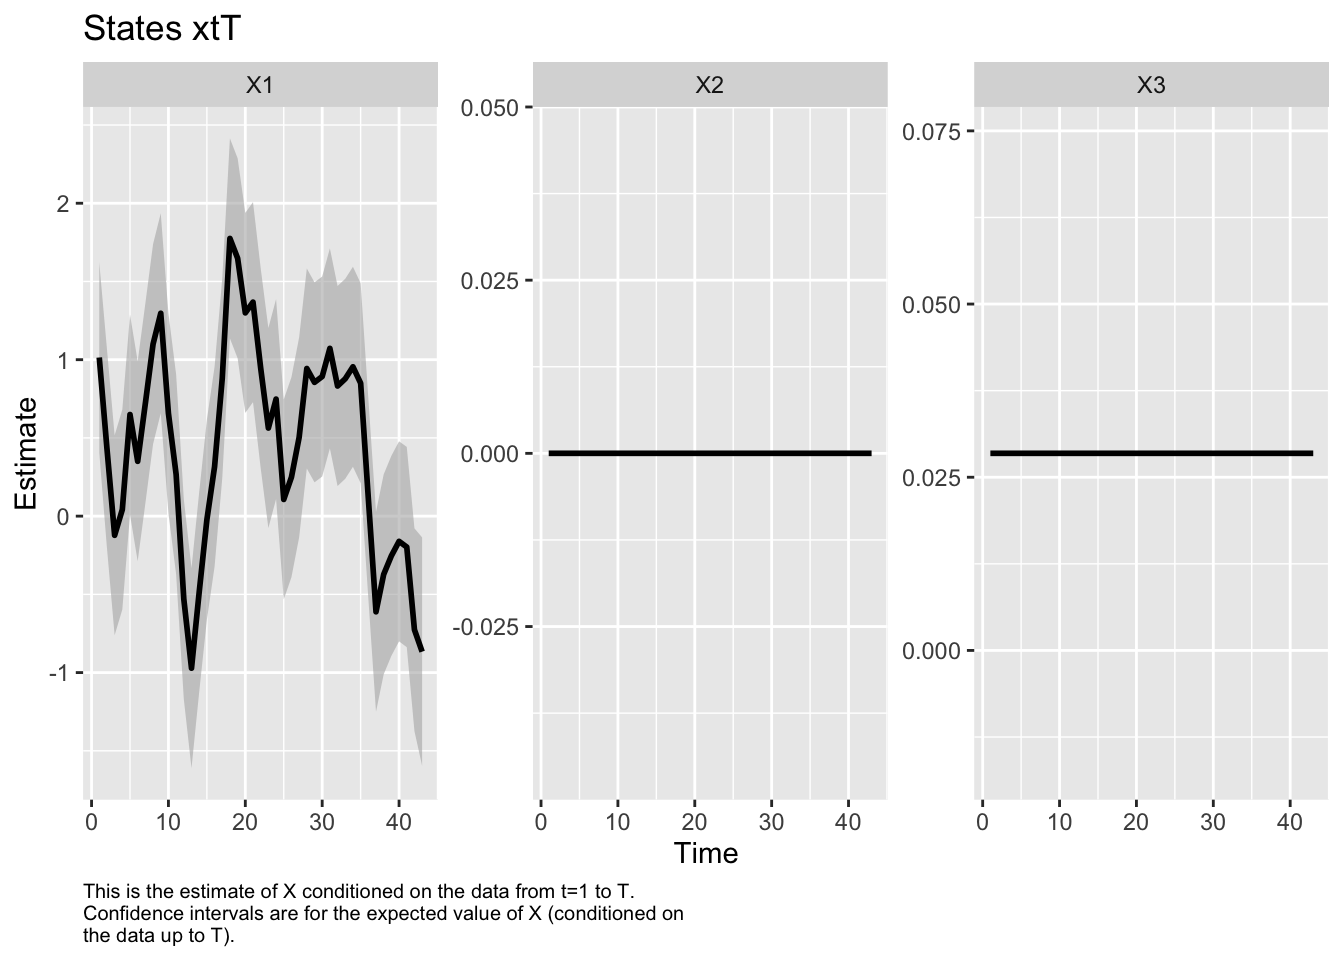
\includegraphics{Lab2-MARSS_files/figure-latex/unnamed-chunk-7-1.pdf}

\begin{Shaded}
\begin{Highlighting}[]
\FunctionTok{plotesu}\NormalTok{(esu[}\DecValTok{4}\NormalTok{])}
\end{Highlighting}
\end{Shaded}

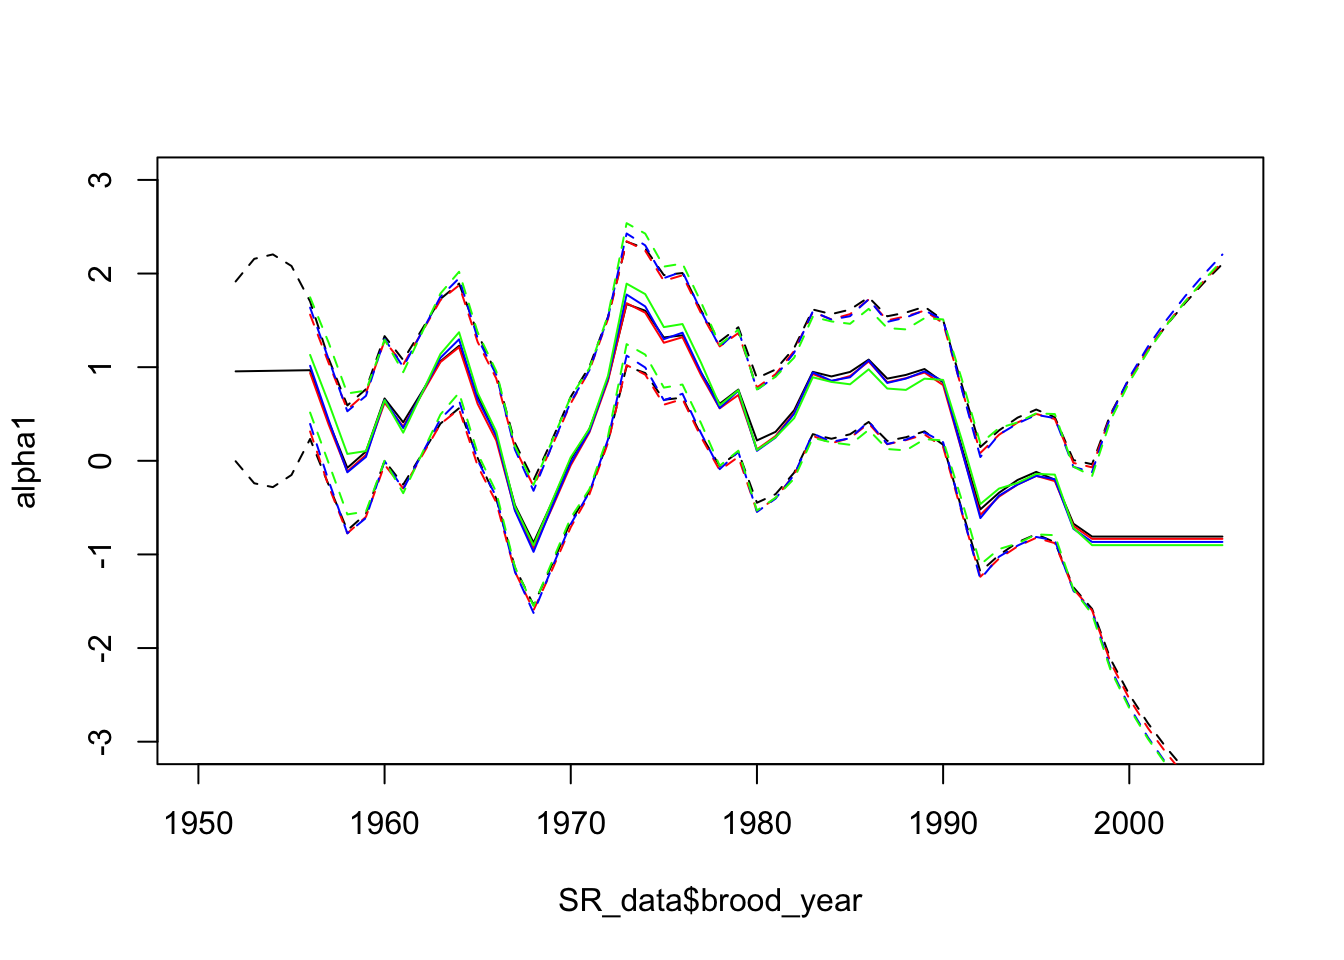
\includegraphics{Lab2-MARSS_files/figure-latex/unnamed-chunk-8-1.pdf}

\begin{Shaded}
\begin{Highlighting}[]
\FunctionTok{plotesu}\NormalTok{(esu[}\DecValTok{5}\NormalTok{])}
\end{Highlighting}
\end{Shaded}

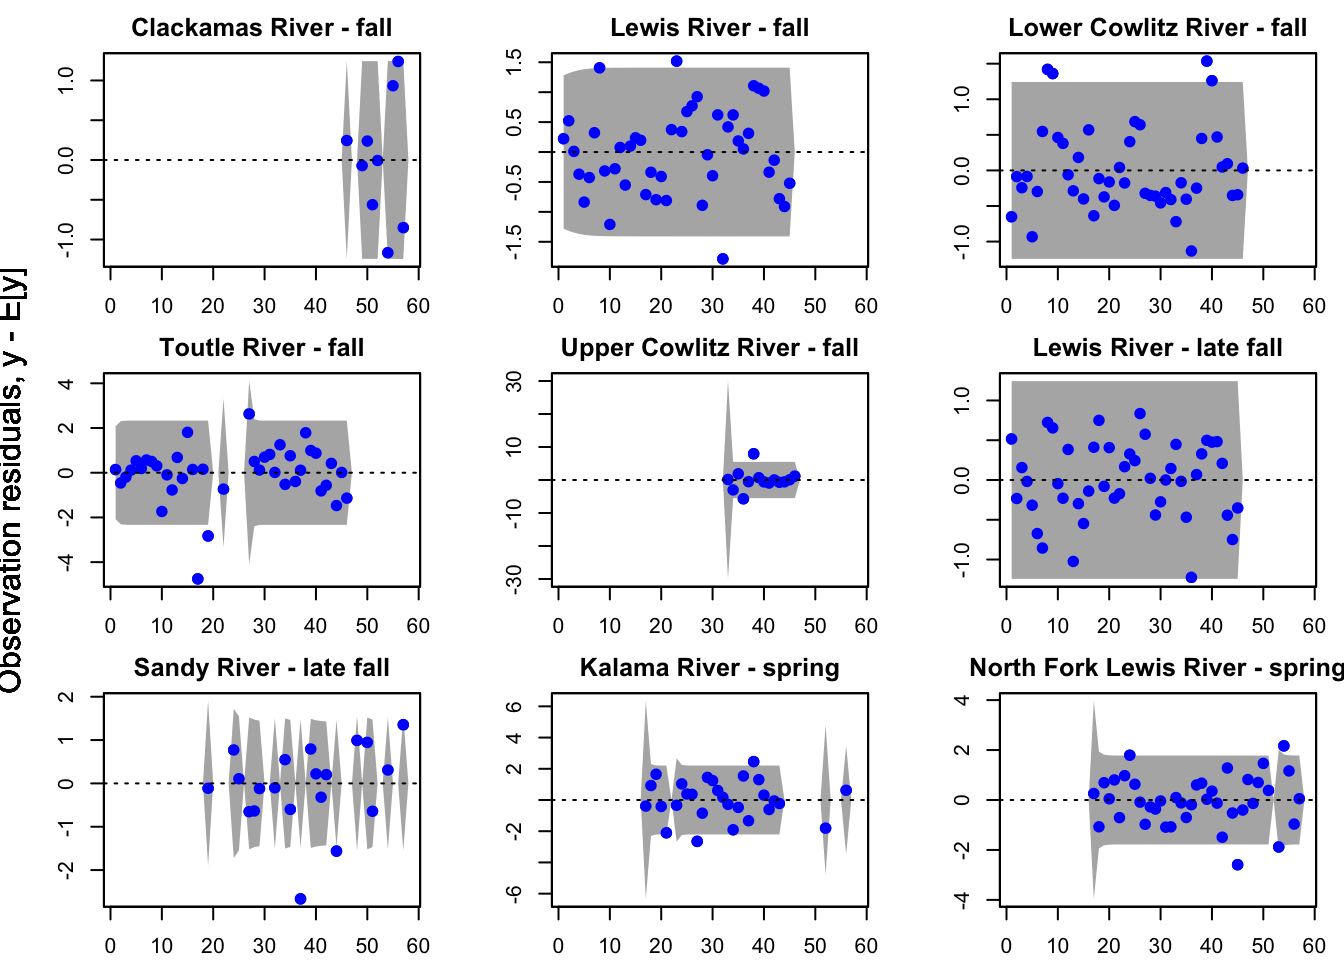
\includegraphics{Lab2-MARSS_files/figure-latex/unnamed-chunk-9-1.pdf}

\begin{Shaded}
\begin{Highlighting}[]
\FunctionTok{plotesu}\NormalTok{(esu[}\DecValTok{1}\NormalTok{])}
\end{Highlighting}
\end{Shaded}

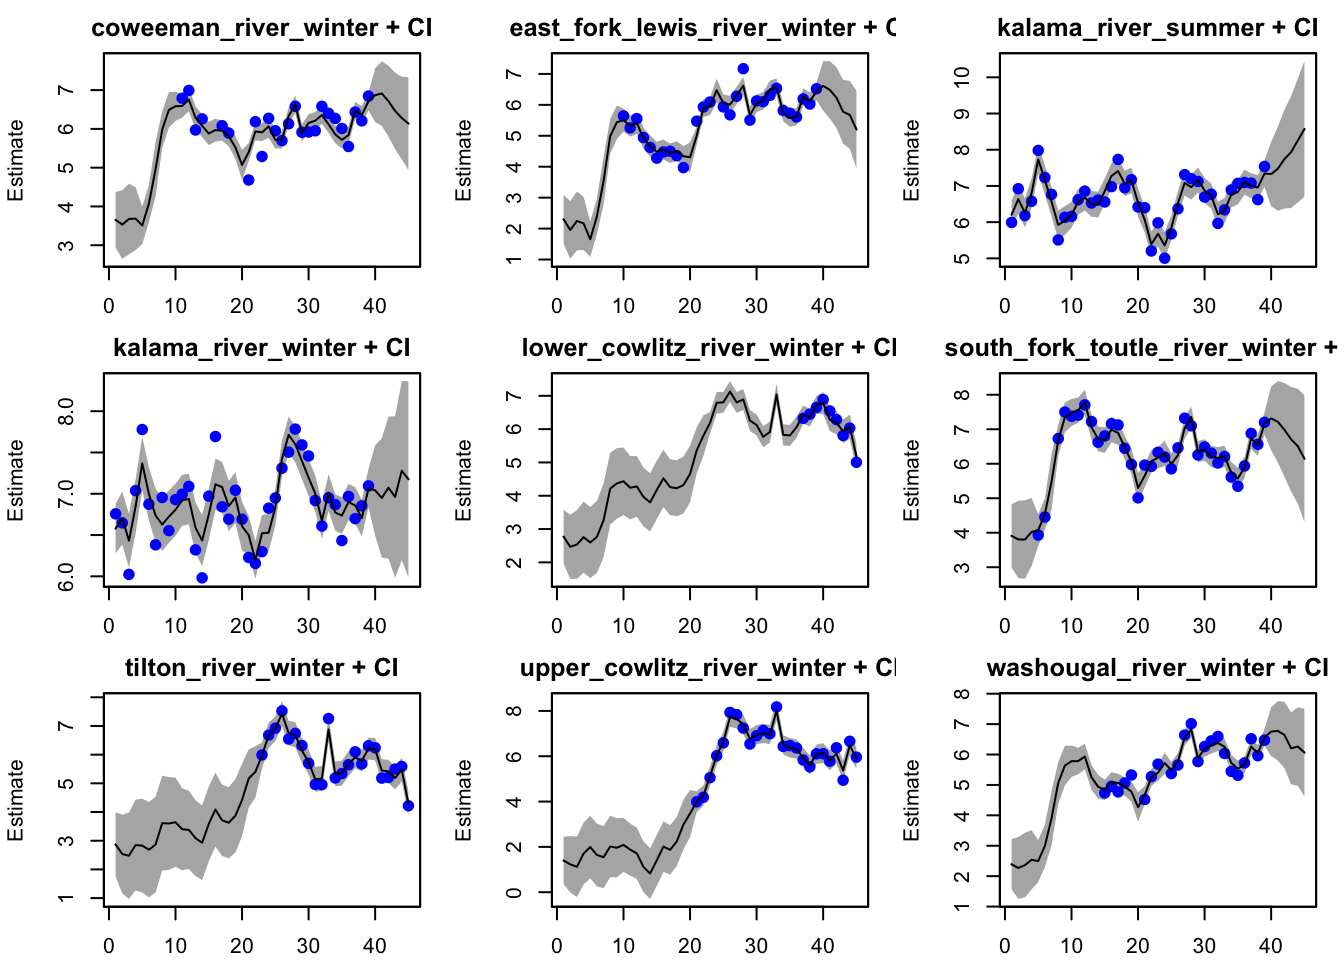
\includegraphics{Lab2-MARSS_files/figure-latex/unnamed-chunk-10-1.pdf}

\begin{Shaded}
\begin{Highlighting}[]
\NormalTok{df }\OtherTok{\textless{}{-}}\NormalTok{ columbia.river }\SpecialCharTok{\%\textgreater{}\%} \FunctionTok{subset}\NormalTok{(species }\SpecialCharTok{==} \StringTok{"Chinook salmon"}\NormalTok{)}
\FunctionTok{ggplot}\NormalTok{(df, }\FunctionTok{aes}\NormalTok{(}\AttributeTok{x=}\NormalTok{spawningyear, }\AttributeTok{y=}\FunctionTok{log}\NormalTok{(value), }\AttributeTok{color=}\NormalTok{run)) }\SpecialCharTok{+} 
  \FunctionTok{geom\_point}\NormalTok{(}\AttributeTok{size=}\FloatTok{0.2}\NormalTok{, }\AttributeTok{na.rm =} \ConstantTok{TRUE}\NormalTok{) }\SpecialCharTok{+}
  \FunctionTok{theme}\NormalTok{(}\AttributeTok{strip.text.x =} \FunctionTok{element\_text}\NormalTok{(}\AttributeTok{size =} \DecValTok{3}\NormalTok{)) }\SpecialCharTok{+}
  \FunctionTok{theme}\NormalTok{(}\AttributeTok{axis.text.x =} \FunctionTok{element\_text}\NormalTok{(}\AttributeTok{size =} \DecValTok{5}\NormalTok{, }\AttributeTok{angle =} \DecValTok{90}\NormalTok{)) }\SpecialCharTok{+} 
  \FunctionTok{facet\_wrap}\NormalTok{(}\SpecialCharTok{\textasciitilde{}}\NormalTok{esapopname)}
\end{Highlighting}
\end{Shaded}

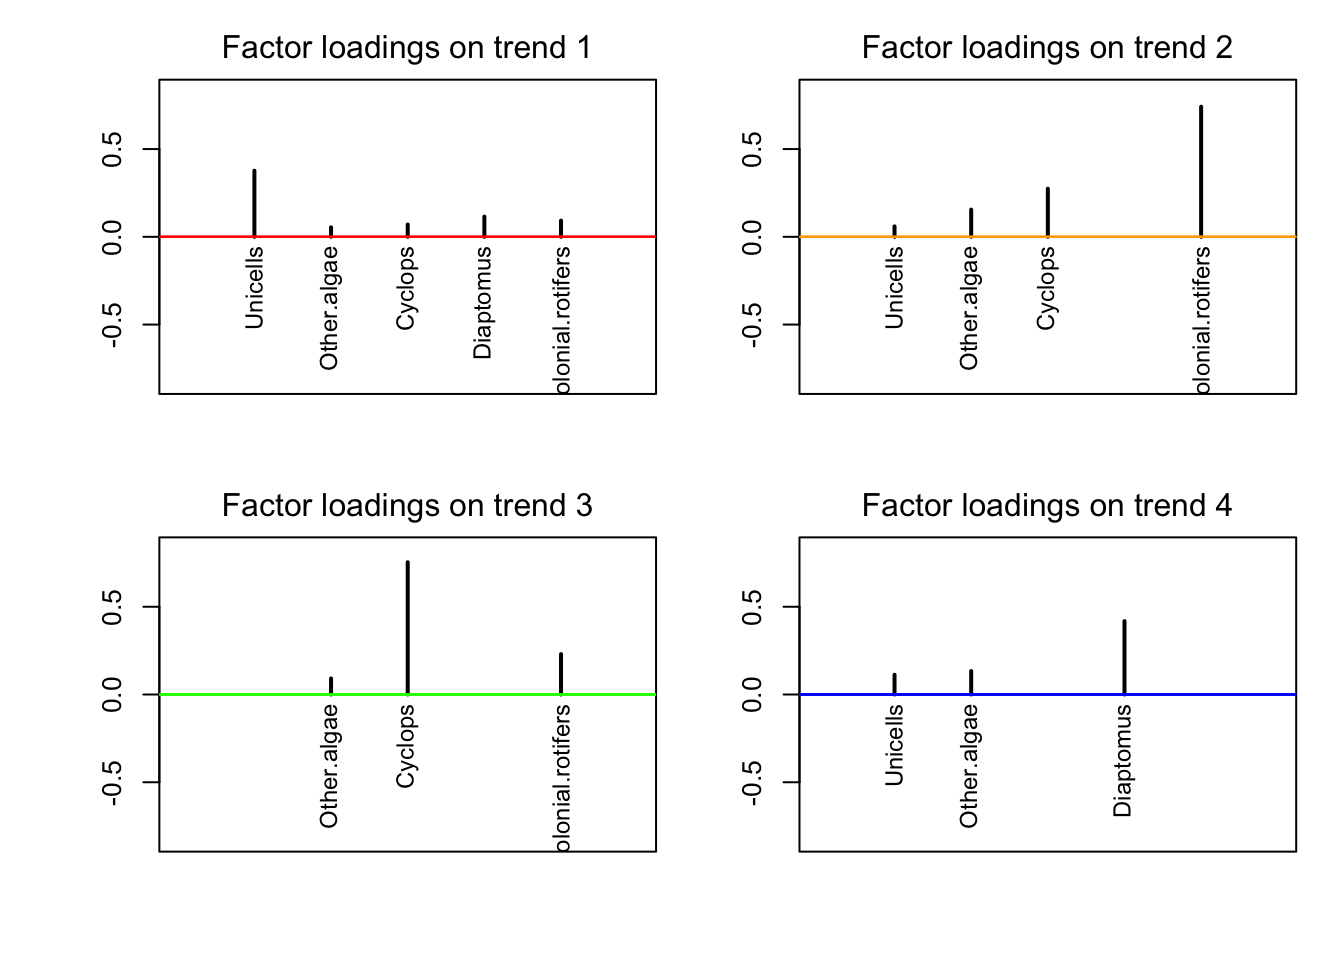
\includegraphics{Lab2-MARSS_files/figure-latex/unnamed-chunk-11-1.pdf}

\hypertarget{tasks-for-each-group}{%
\subsection{Tasks for each group}\label{tasks-for-each-group}}

\begin{enumerate}
\def\labelenumi{\arabic{enumi}.}
\item
  Create estimates of spawner abundance for all missing years and
  provide estimates of the decline from the historical abundance.
\item
  Evaluate support for the major population groups. Are the populations
  in the groups more correlated than outside the groups?
\item
  Evaluate the evidence of cycling in the data. \emph{We will talk about
  how to do this on the Tuesday after lab.}
\end{enumerate}

\hypertarget{tips}{%
\subsubsection{Tips}\label{tips}}

\textbf{Simplify}

If your ESU has many populations, start with a smaller set of 4-7
populations.

\textbf{Assumptions}

You can assume that \texttt{R="diagonal\ and\ equal"} and
\texttt{A="scaling"}. Assume that ``historical'' means the earliest
years available for your group.

\textbf{States}

Your abundance estimate is the ``x'' or ``state'' estimates. You can get
this from

\begin{verbatim}
fit$states
\end{verbatim}

or

\begin{verbatim}
tsSmooth(fit)
\end{verbatim}

where \texttt{fit} is from \texttt{fit\ \textless{}-\ MARSS()}

\textbf{plotting}

Estimate of the mean of the spawner counts based on your x model.

\begin{verbatim}
autoplot(fit, plot.type="fitted.ytT")
\end{verbatim}

\textbf{diagnostics}

\begin{verbatim}
autoplot(fit, plot.type="residuals")
\end{verbatim}

\hypertarget{address-the-following-in-your-methods}{%
\subsubsection{Address the following in your
methods}\label{address-the-following-in-your-methods}}

\begin{itemize}
\item
  Describe your assumptions about the x and how the data time series are
  related to x.

  \begin{itemize}
  \tightlist
  \item
    How are the x and y (data) related? 1 x for 1 y or will you assume 1
    x for all y or 1 x for each major population group? How will you
    choose?
  \item
    What will you assume about the U for the x's?
  \item
    What will you assume about the Q matrix?
  \end{itemize}
\item
  Write out your assumptions as different models \textbf{in matrix
  form}, fit each and then compare these with AIC or AICc.
\item
  Do your estimates differ depending on the assumptions you make about
  the structure of the data, i.e.~you assumptions about the x's, Q, and
  U.
\end{itemize}

\hypertarget{sample-code}{%
\subsection{Sample code}\label{sample-code}}

Here I show how I might analyze the Upper Columbia Steelhead data.

\begin{figure}
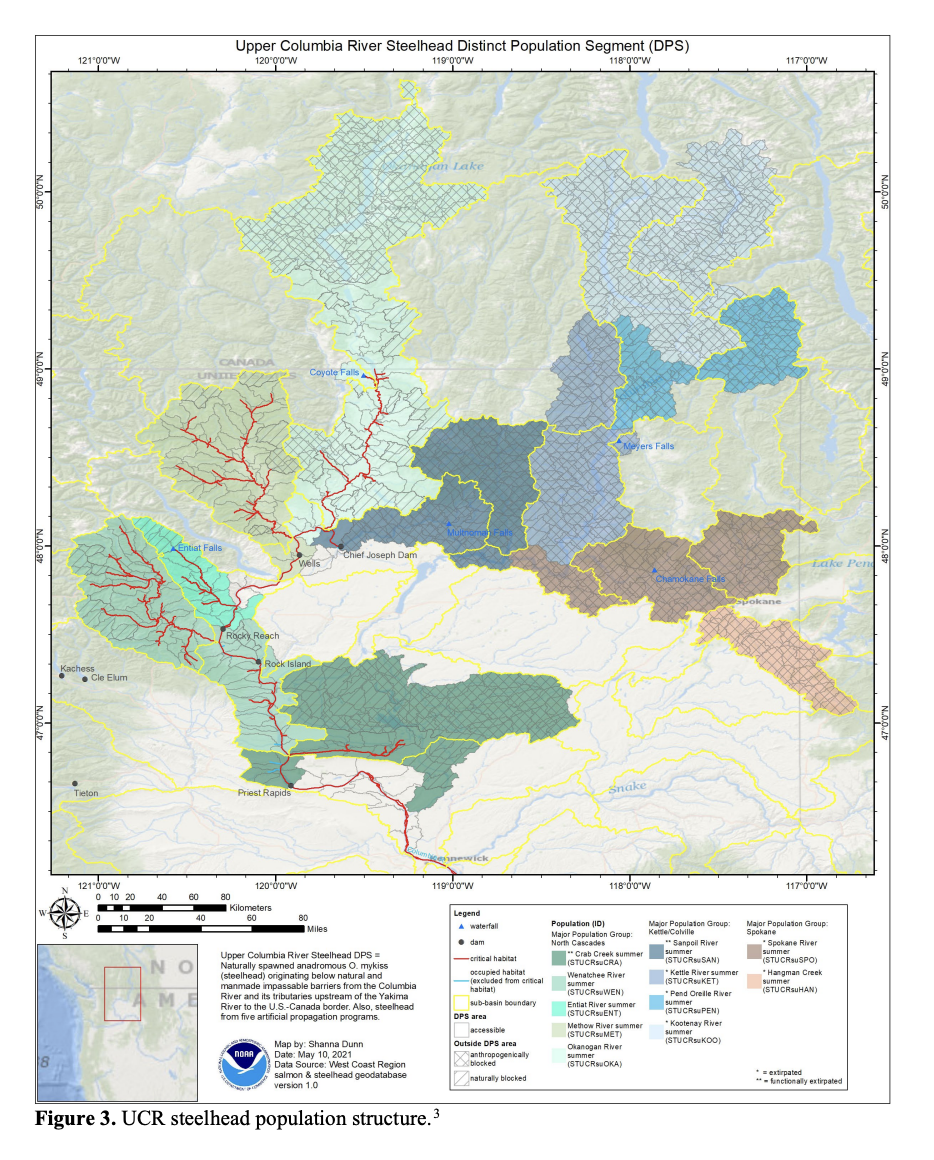
\includegraphics[width=0.5\linewidth]{Data_Images/UCR-Steelhead-regions} \caption{Figure from 2022 5-Year Review: Summary & Evaluation of Upper Columbia River Spring-run Chinook Salmon and Upper Columbia River Steelhead. NMFS. West Coast Region. https://doi.org/10.25923/p4w5-dp31}\label{fig:unnamed-chunk-12}
\end{figure}

Set up the data. We need the time series in a matrix with time across
the columns.

Load the data.

\begin{Shaded}
\begin{Highlighting}[]
\FunctionTok{load}\NormalTok{(here}\SpecialCharTok{::}\FunctionTok{here}\NormalTok{(}\StringTok{"Lab{-}2"}\NormalTok{, }\StringTok{"Data\_Images"}\NormalTok{, }\StringTok{"columbia{-}river.rda"}\NormalTok{))}
\end{Highlighting}
\end{Shaded}

Wrangle the data.

\begin{Shaded}
\begin{Highlighting}[]
\FunctionTok{library}\NormalTok{(dplyr)}
\NormalTok{esuname }\OtherTok{\textless{}{-}}\NormalTok{ esu[}\DecValTok{2}\NormalTok{]}

\NormalTok{dat }\OtherTok{\textless{}{-}}\NormalTok{ columbia.river }\SpecialCharTok{\%\textgreater{}\%} 
  \FunctionTok{subset}\NormalTok{(esu\_dps }\SpecialCharTok{==}\NormalTok{ esuname) }\SpecialCharTok{\%\textgreater{}\%} \CommentTok{\# get only this ESU}
  \FunctionTok{mutate}\NormalTok{(}\AttributeTok{log.spawner =} \FunctionTok{log}\NormalTok{(value)) }\SpecialCharTok{\%\textgreater{}\%} \CommentTok{\# create a column called log.spawner}
  \FunctionTok{select}\NormalTok{(esapopname, spawningyear, log.spawner) }\SpecialCharTok{\%\textgreater{}\%} \CommentTok{\# get just the columns that I need}
  \FunctionTok{pivot\_wider}\NormalTok{(}\AttributeTok{names\_from =} \StringTok{"esapopname"}\NormalTok{, }\AttributeTok{values\_from =} \StringTok{"log.spawner"}\NormalTok{) }\SpecialCharTok{\%\textgreater{}\%} 
  \FunctionTok{column\_to\_rownames}\NormalTok{(}\AttributeTok{var =} \StringTok{"spawningyear"}\NormalTok{) }\SpecialCharTok{\%\textgreater{}\%} \CommentTok{\# make the years rownames}
  \FunctionTok{as.matrix}\NormalTok{() }\SpecialCharTok{\%\textgreater{}\%} \CommentTok{\# turn into a matrix with year down the rows}
  \FunctionTok{t}\NormalTok{() }\CommentTok{\# make time across the columns}
\CommentTok{\# MARSS complains if I don\textquotesingle{}t do this}
\NormalTok{dat[}\FunctionTok{is.na}\NormalTok{(dat)] }\OtherTok{\textless{}{-}} \ConstantTok{NA}
\end{Highlighting}
\end{Shaded}

Clean up the row names

\begin{Shaded}
\begin{Highlighting}[]
\NormalTok{tmp }\OtherTok{\textless{}{-}} \FunctionTok{rownames}\NormalTok{(dat)}
\NormalTok{tmp }\OtherTok{\textless{}{-}}\NormalTok{ stringr}\SpecialCharTok{::}\FunctionTok{str\_replace}\NormalTok{(tmp, }\StringTok{"Steelhead [(]Upper Columbia River DPS[)]"}\NormalTok{, }\StringTok{""}\NormalTok{)}
\NormalTok{tmp }\OtherTok{\textless{}{-}}\NormalTok{ stringr}\SpecialCharTok{::}\FunctionTok{str\_replace}\NormalTok{(tmp, }\StringTok{"River {-} summer"}\NormalTok{, }\StringTok{""}\NormalTok{)}
\NormalTok{tmp }\OtherTok{\textless{}{-}}\NormalTok{ stringr}\SpecialCharTok{::}\FunctionTok{str\_trim}\NormalTok{(tmp)}
\FunctionTok{rownames}\NormalTok{(dat) }\OtherTok{\textless{}{-}}\NormalTok{ tmp}
\end{Highlighting}
\end{Shaded}

Specify a model

\begin{Shaded}
\begin{Highlighting}[]
\NormalTok{mod.list1 }\OtherTok{\textless{}{-}} \FunctionTok{list}\NormalTok{(}
  \AttributeTok{U =} \StringTok{"unequal"}\NormalTok{,}
  \AttributeTok{R =} \StringTok{"diagonal and equal"}\NormalTok{,}
  \AttributeTok{Q =} \StringTok{"unconstrained"}
\NormalTok{)}
\end{Highlighting}
\end{Shaded}

Fit the model. In this case, a BFGS algorithm is faster.

\begin{Shaded}
\begin{Highlighting}[]
\FunctionTok{library}\NormalTok{(MARSS)}
\NormalTok{fit1 }\OtherTok{\textless{}{-}} \FunctionTok{MARSS}\NormalTok{(dat, }\AttributeTok{model=}\NormalTok{mod.list1, }\AttributeTok{method=}\StringTok{"BFGS"}\NormalTok{)}
\end{Highlighting}
\end{Shaded}

\begin{verbatim}
## Success! Converged in 235 iterations.
## Function MARSSkfas used for likelihood calculation.
## 
## MARSS fit is
## Estimation method: BFGS 
## Estimation converged in 235 iterations. 
## Log-likelihood: -109.4078 
## AIC: 256.8155   AICc: 262.1676   
##  
##                Estimate
## R.diag          0.00997
## U.X.Entiat      0.02182
## U.X.Methow      0.01852
## U.X.Okanogan    0.00140
## U.X.Wenatchee  -0.02222
## Q.(1,1)         0.28016
## Q.(2,1)         0.12303
## Q.(3,1)         0.14275
## Q.(4,1)         0.23415
## Q.(2,2)         0.31642
## Q.(3,2)         0.30806
## Q.(4,2)         0.19061
## Q.(3,3)         0.31031
## Q.(4,3)         0.18852
## Q.(4,4)         0.52813
## x0.X.Entiat     4.61643
## x0.X.Methow     6.43404
## x0.X.Okanogan   6.47218
## x0.X.Wenatchee  8.04871
## Initial states (x0) defined at t=0
## 
## Standard errors have not been calculated. 
## Use MARSSparamCIs to compute CIs and bias estimates.
\end{verbatim}

Hmmmmm, the Q variance is so high that it perfectly fits the data. That
doesn't seem right.

\begin{Shaded}
\begin{Highlighting}[]
\FunctionTok{autoplot}\NormalTok{(fit1, }\AttributeTok{plot.type=}\StringTok{"fitted.ytT"}\NormalTok{)}
\end{Highlighting}
\end{Shaded}

\begin{verbatim}
## MARSSresiduals.tT reported warnings. See msg element or attribute of returned residuals object.
\end{verbatim}

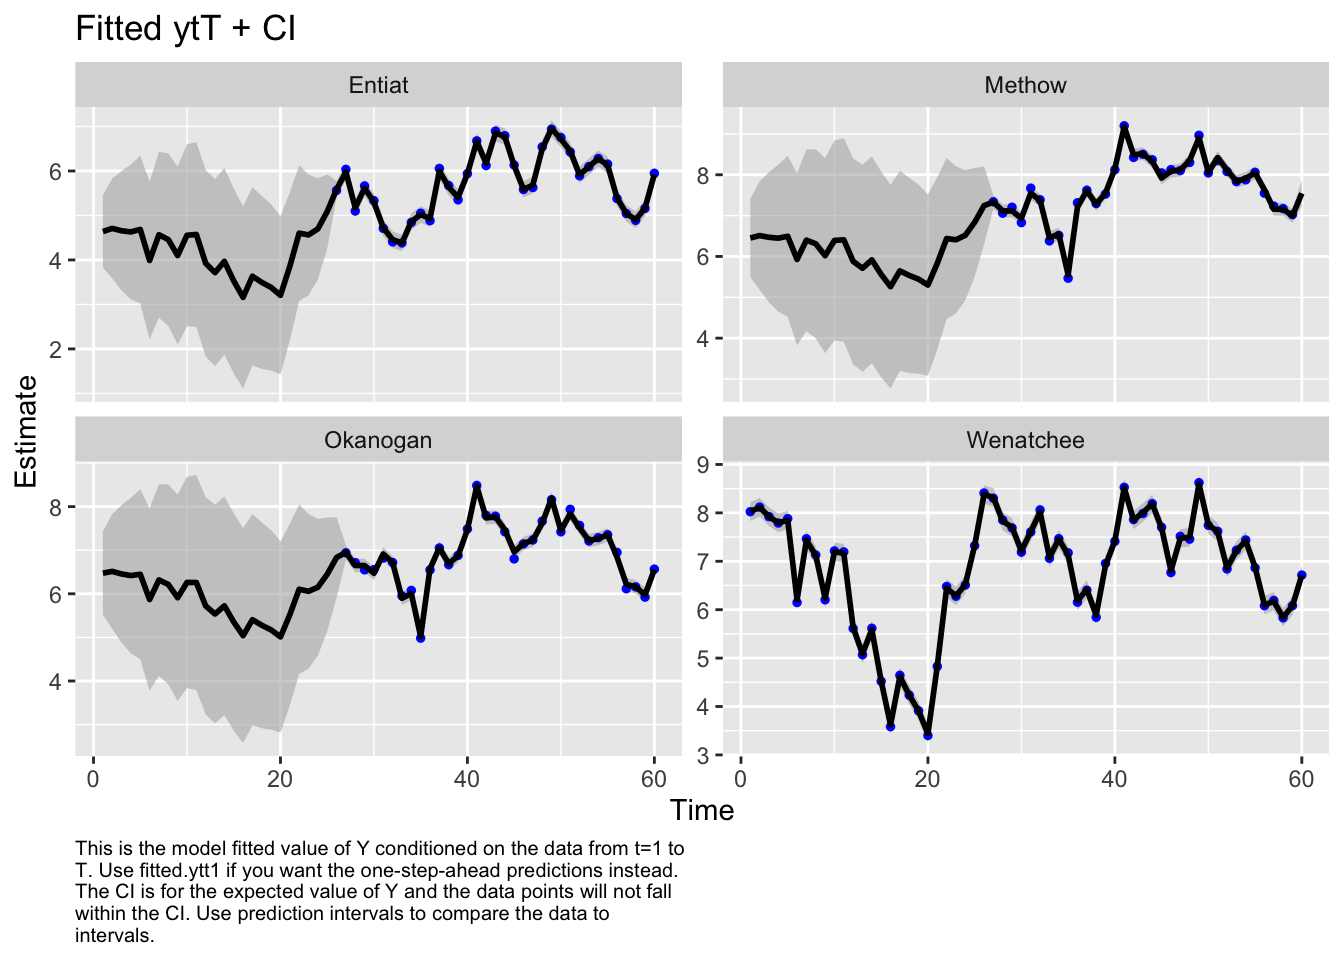
\includegraphics{Lab2-MARSS_files/figure-latex/unnamed-chunk-18-1.pdf}

\begin{verbatim}
## plot.type = fitted.ytT
\end{verbatim}

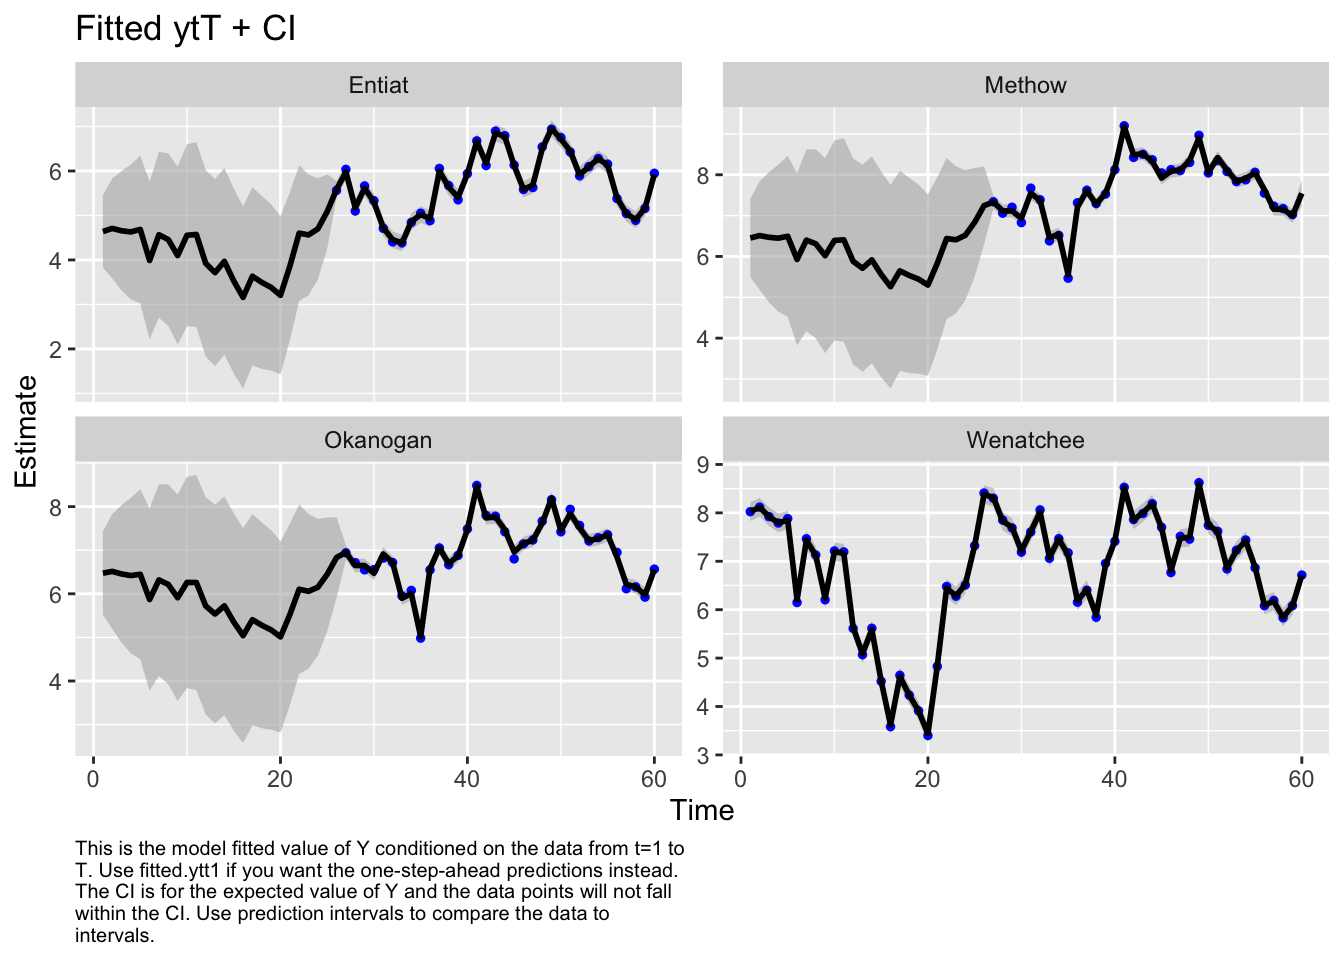
\includegraphics{Lab2-MARSS_files/figure-latex/unnamed-chunk-18-2.pdf}

\begin{verbatim}
## Finished plots.
\end{verbatim}

Let's look at the corrplot. Interesting. The Methow and Entiat are
almost perfectly correlated while the Entiat and Wenatchee are somewhat
correlated. That makes sense if you look at a map.

\begin{Shaded}
\begin{Highlighting}[]
\FunctionTok{library}\NormalTok{(corrplot)}
\end{Highlighting}
\end{Shaded}

\begin{verbatim}
## corrplot 0.92 loaded
\end{verbatim}

\begin{Shaded}
\begin{Highlighting}[]
\NormalTok{Q }\OtherTok{\textless{}{-}} \FunctionTok{coef}\NormalTok{(fit1, }\AttributeTok{type=}\StringTok{"matrix"}\NormalTok{)}\SpecialCharTok{$}\NormalTok{Q}
\NormalTok{corrmat }\OtherTok{\textless{}{-}} \FunctionTok{diag}\NormalTok{(}\DecValTok{1}\SpecialCharTok{/}\FunctionTok{sqrt}\NormalTok{(}\FunctionTok{diag}\NormalTok{(Q))) }\SpecialCharTok{\%*\%}\NormalTok{ Q }\SpecialCharTok{\%*\%} \FunctionTok{diag}\NormalTok{(}\DecValTok{1}\SpecialCharTok{/}\FunctionTok{sqrt}\NormalTok{(}\FunctionTok{diag}\NormalTok{(Q)))}
\FunctionTok{corrplot}\NormalTok{(corrmat)}
\end{Highlighting}
\end{Shaded}

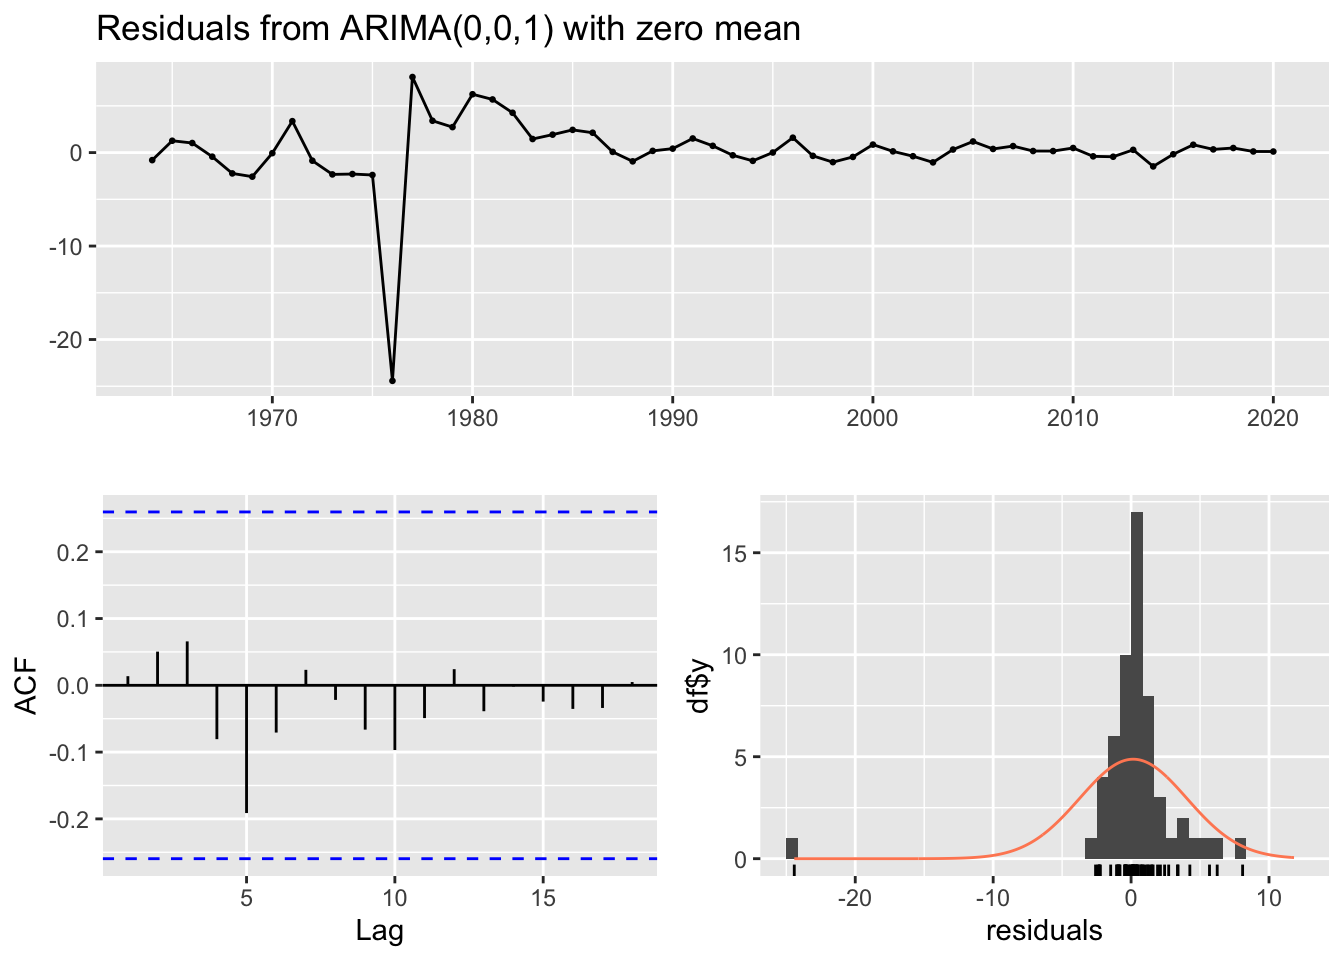
\includegraphics{Lab2-MARSS_files/figure-latex/unnamed-chunk-19-1.pdf}

I need to use the EM algorithm (remove \texttt{method="BFGS"}) because
the BFGS algorithm doesn't allow constraints on the Q matrix.

\begin{Shaded}
\begin{Highlighting}[]
\NormalTok{mod.list2 }\OtherTok{\textless{}{-}} \FunctionTok{list}\NormalTok{(}
  \AttributeTok{U =} \StringTok{"unequal"}\NormalTok{,}
  \AttributeTok{R =} \StringTok{"diagonal and equal"}\NormalTok{,}
  \AttributeTok{Q =} \StringTok{"equalvarcov"}
\NormalTok{)}
\NormalTok{fit2 }\OtherTok{\textless{}{-}} \FunctionTok{MARSS}\NormalTok{(dat, }\AttributeTok{model=}\NormalTok{mod.list2, }\AttributeTok{control =} \FunctionTok{list}\NormalTok{(}\AttributeTok{maxit=}\DecValTok{1000}\NormalTok{))}
\end{Highlighting}
\end{Shaded}

\begin{verbatim}
## Success! abstol and log-log tests passed at 794 iterations.
## Alert: conv.test.slope.tol is 0.5.
## Test with smaller values (<0.1) to ensure convergence.
## 
## MARSS fit is
## Estimation method: kem 
## Convergence test: conv.test.slope.tol = 0.5, abstol = 0.001
## Estimation converged in 794 iterations. 
## Log-likelihood: -120.6028 
## AIC: 263.2057   AICc: 264.9657   
##  
##                Estimate
## R.diag           0.1290
## U.X.Entiat       0.0257
## U.X.Methow       0.0311
## U.X.Okanogan     0.0166
## U.X.Wenatchee   -0.0282
## Q.diag           0.2632
## Q.offdiag        0.2631
## x0.X.Entiat      4.2026
## x0.X.Methow      5.9042
## x0.X.Okanogan    5.8359
## x0.X.Wenatchee   8.0703
## Initial states (x0) defined at t=0
## 
## Standard errors have not been calculated. 
## Use MARSSparamCIs to compute CIs and bias estimates.
\end{verbatim}

\begin{Shaded}
\begin{Highlighting}[]
\FunctionTok{autoplot}\NormalTok{(fit2, }\AttributeTok{plot.type=}\StringTok{"fitted.ytT"}\NormalTok{)}
\end{Highlighting}
\end{Shaded}

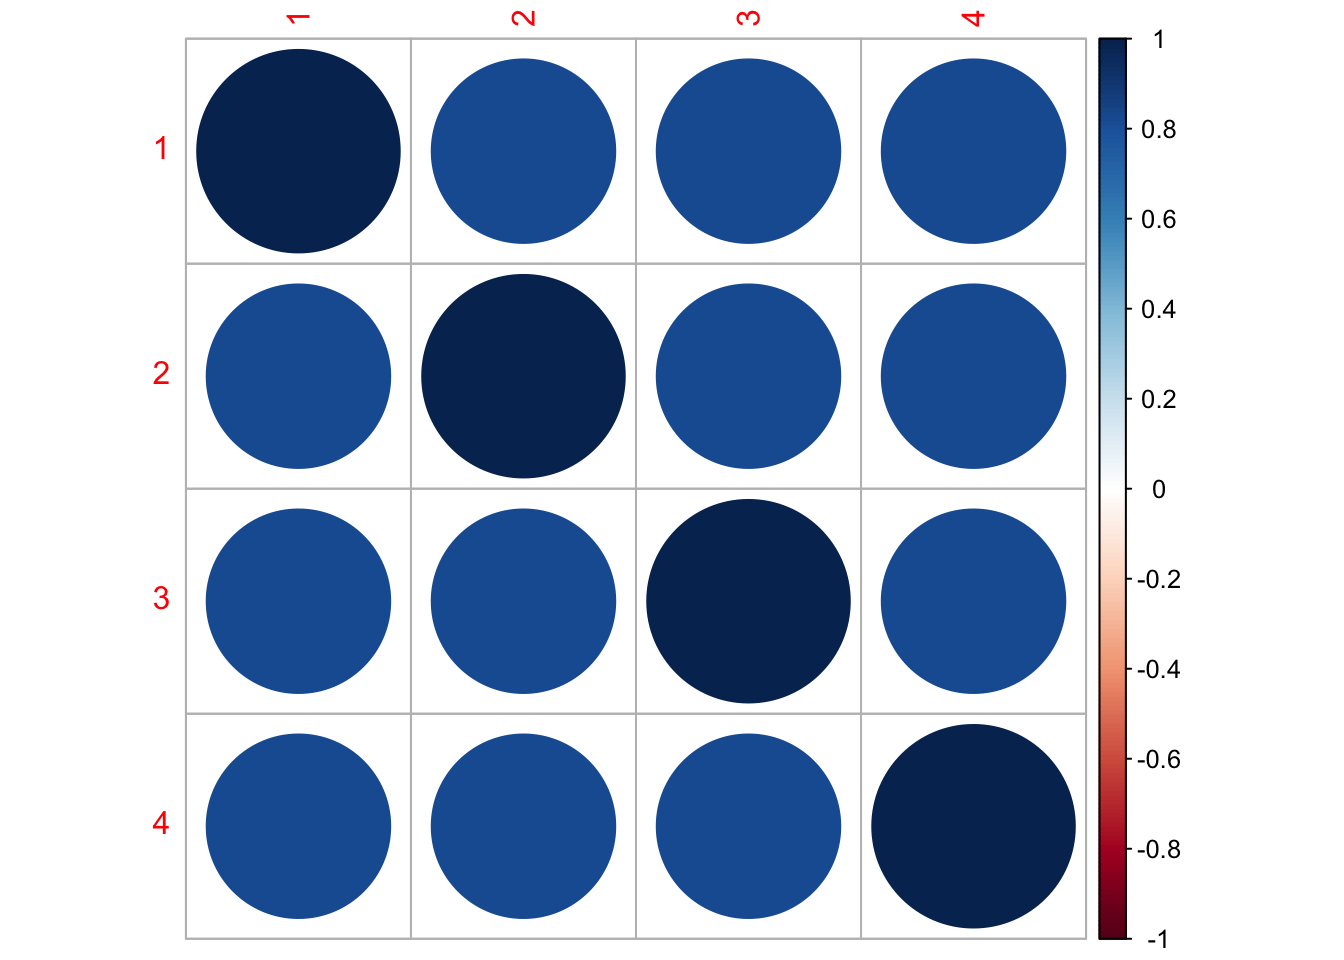
\includegraphics{Lab2-MARSS_files/figure-latex/unnamed-chunk-21-1.pdf}

\begin{verbatim}
## plot.type = fitted.ytT
\end{verbatim}

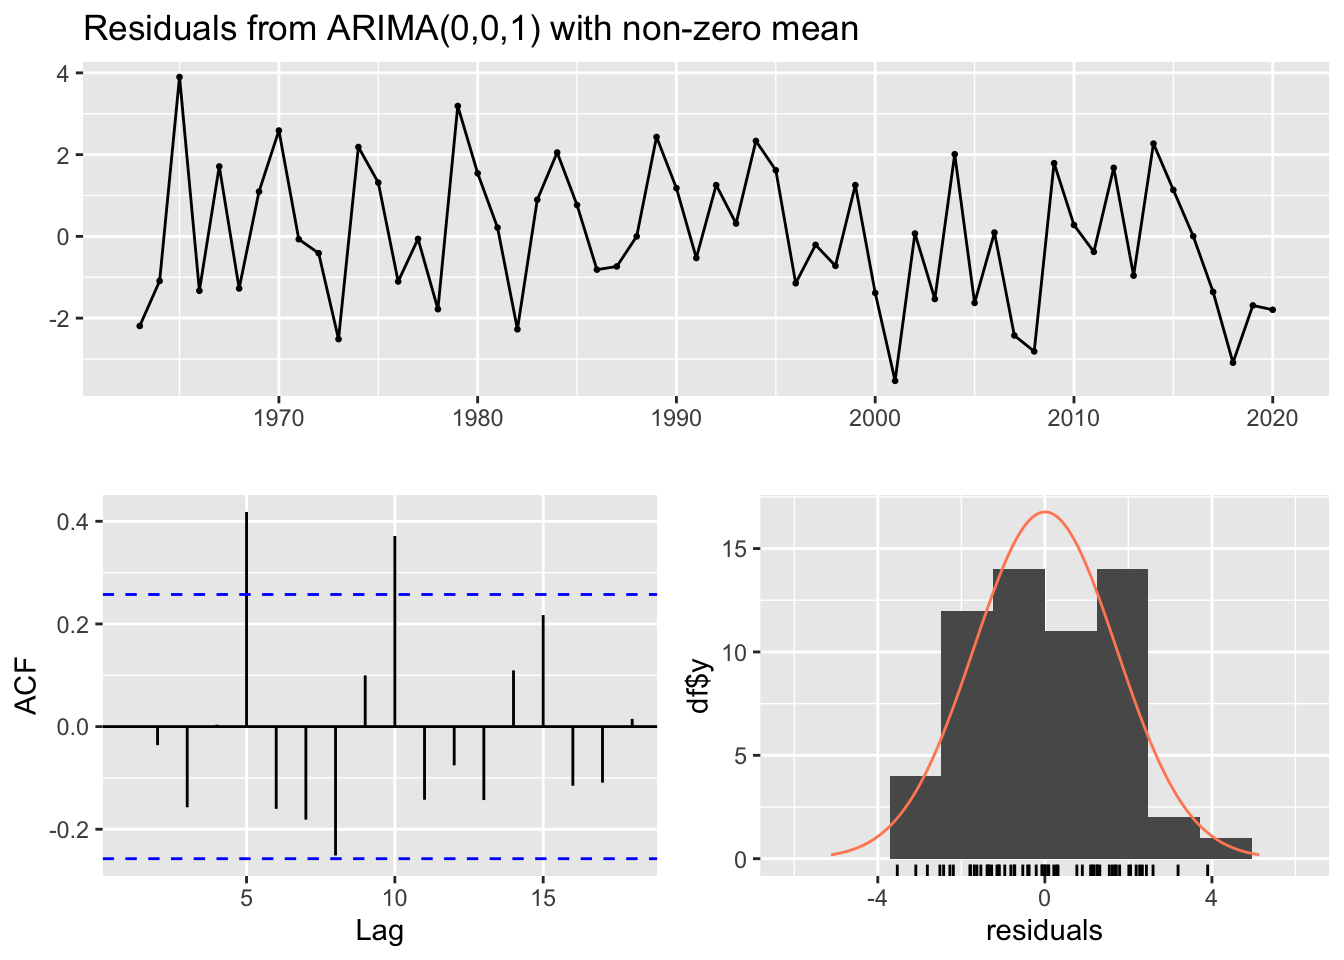
\includegraphics{Lab2-MARSS_files/figure-latex/unnamed-chunk-21-2.pdf}

\begin{verbatim}
## Finished plots.
\end{verbatim}

Now I want try something different. I will treat the Methow-Okanogan as
one state and the Entiat-Wenatchee as another. I'll let these be
correlated together. Interesting, these two are estimated to be
perfectly correlated.

\begin{Shaded}
\begin{Highlighting}[]
\NormalTok{mod.list3 }\OtherTok{\textless{}{-}}\NormalTok{ mod.list1}
\NormalTok{mod.list3}\SpecialCharTok{$}\NormalTok{Q }\OtherTok{\textless{}{-}} \StringTok{"unconstrained"}
\NormalTok{mod.list3}\SpecialCharTok{$}\NormalTok{Z }\OtherTok{\textless{}{-}} \FunctionTok{factor}\NormalTok{(}\FunctionTok{c}\NormalTok{(}\StringTok{"ew"}\NormalTok{, }\StringTok{"mo"}\NormalTok{, }\StringTok{"mo"}\NormalTok{, }\StringTok{"ew"}\NormalTok{))}
\NormalTok{fit3 }\OtherTok{\textless{}{-}} \FunctionTok{MARSS}\NormalTok{(dat, }\AttributeTok{model =}\NormalTok{ mod.list3)}
\end{Highlighting}
\end{Shaded}

\begin{verbatim}
## Warning! Reached maxit before parameters converged. Maxit was 500.
##  neither abstol nor log-log convergence tests were passed.
## 
## MARSS fit is
## Estimation method: kem 
## Convergence test: conv.test.slope.tol = 0.5, abstol = 0.001
## WARNING: maxit reached at  500  iter before convergence.
##  Neither abstol nor log-log convergence test were passed.
##  The likelihood and params are not at the ML values.
##  Try setting control$maxit higher.
## Log-likelihood: -137.532 
## AIC: 295.064   AICc: 296.5209   
##  
##             Estimate
## A.Okanogan  -0.68779
## A.Wenatchee  1.54127
## R.diag       0.18062
## U.ew        -0.02175
## U.mo         0.00374
## Q.(1,1)      0.22050
## Q.(2,1)      0.22103
## Q.(2,2)      0.22164
## x0.ew        6.51468
## x0.mo        7.33795
## Initial states (x0) defined at t=0
## 
## Standard errors have not been calculated. 
## Use MARSSparamCIs to compute CIs and bias estimates.
## 
## Convergence warnings
##  Warning: the  logLik  parameter value has not converged.
##  Type MARSSinfo("convergence") for more info on this warning.
\end{verbatim}

\begin{Shaded}
\begin{Highlighting}[]
\FunctionTok{autoplot}\NormalTok{(fit3, }\AttributeTok{plot.type=}\StringTok{"fitted.ytT"}\NormalTok{)}
\end{Highlighting}
\end{Shaded}

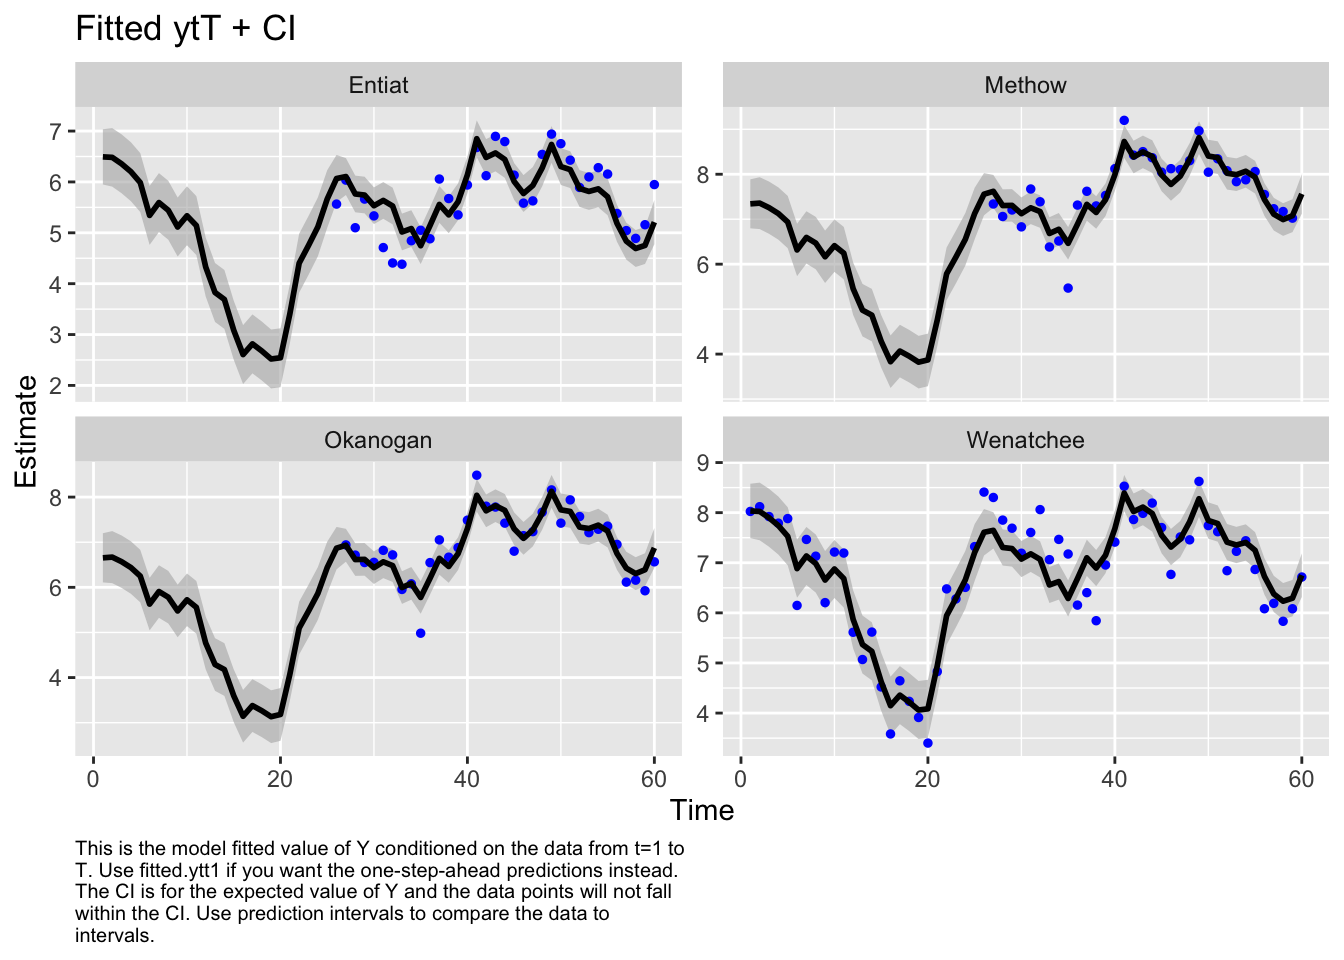
\includegraphics{Lab2-MARSS_files/figure-latex/unnamed-chunk-22-1.pdf}

\begin{verbatim}
## plot.type = fitted.ytT
\end{verbatim}

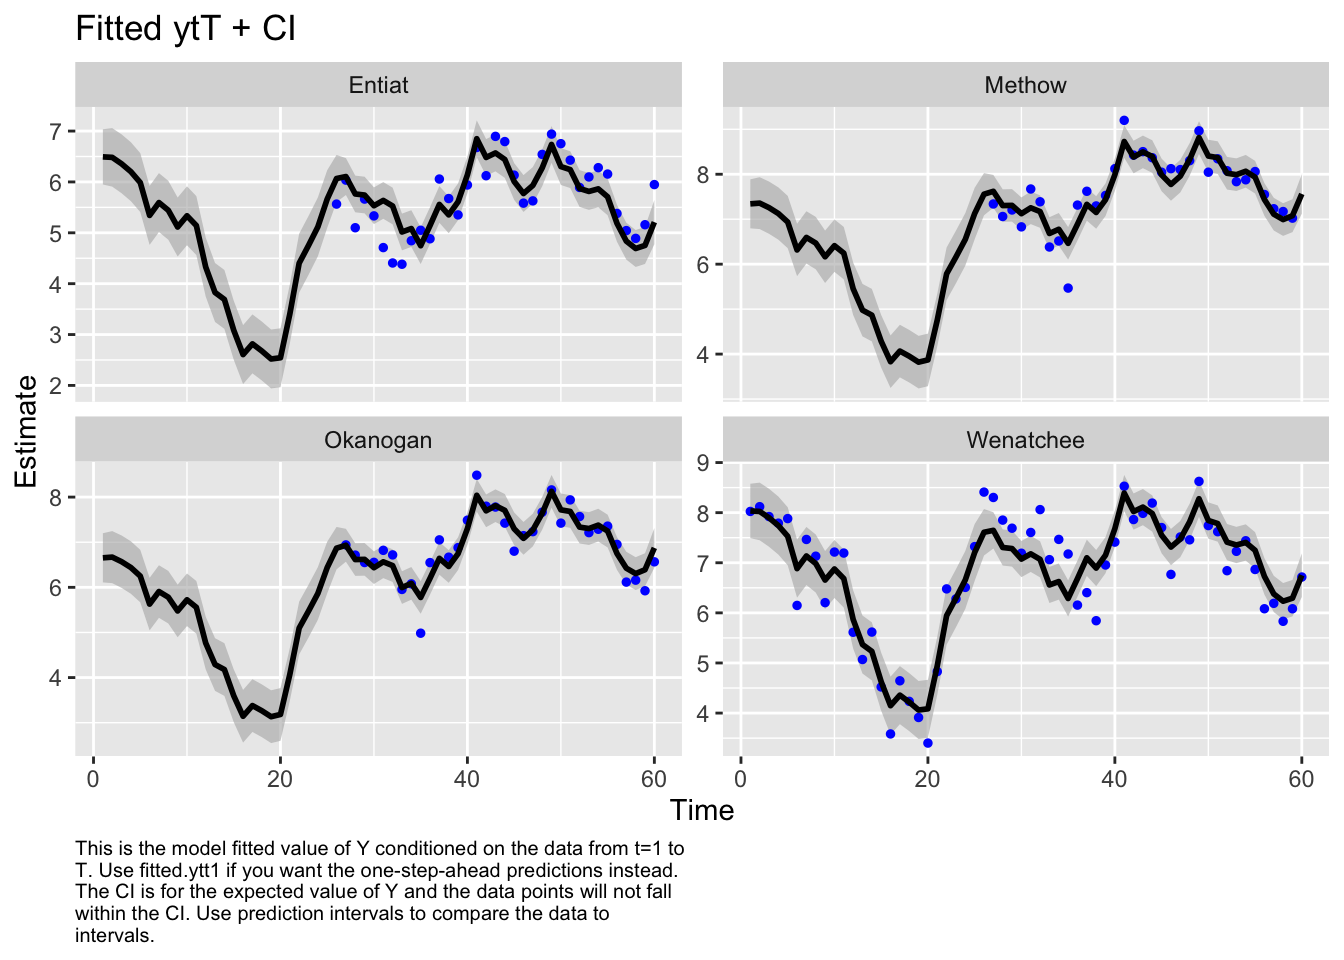
\includegraphics{Lab2-MARSS_files/figure-latex/unnamed-chunk-22-2.pdf}

\begin{verbatim}
## Finished plots.
\end{verbatim}

Finally, let's look at the AIC values. Fit1 was very flexible and can
put a line through the data so I know I have at least one model in the
set that can fit the data. Well, the most flexible model is the best. At
this point, I'd like to look just at data after 1980 or so. I don't like
the big dip that happened in the Wenatchee River. I'd want to talk to
the biologists to find out what happened, especially because I know that
there might be hatchery releases in this system.

\begin{Shaded}
\begin{Highlighting}[]
\NormalTok{aic }\OtherTok{\textless{}{-}} \FunctionTok{c}\NormalTok{(fit1}\SpecialCharTok{$}\NormalTok{AICc, fit2}\SpecialCharTok{$}\NormalTok{AICc, fit3}\SpecialCharTok{$}\NormalTok{AICc)}
\NormalTok{aic}\SpecialCharTok{{-}}\FunctionTok{min}\NormalTok{(aic)}
\end{Highlighting}
\end{Shaded}

\begin{verbatim}
## [1]  0.00000  2.79807 34.35331
\end{verbatim}

\hypertarget{resources}{%
\subsection{Resources}\label{resources}}

Chapter 7 MARSS models. ATSA Lab Book.
\url{https://atsa-es.github.io/atsa-labs/chap-mss.html}

Chapter 8 MARSS models with covariate. ATSA Lab Book.
\url{https://atsa-es.github.io/atsa-labs/chap-msscov.html}

Chapter 16 Modeling cyclic sockeye
\url{https://atsa-es.github.io/atsa-labs/chap-cyclic-sockeye.html}

\end{document}
